\documentclass[a4paper]{article}
\usepackage{header}

\usepackage{tikz}
\usepackage{tikz-network}
\usepackage{float}

\newcommand\enumtocitem[3]{\item\textbf{#1}\addtocounter{#2}{1}\addcontentsline{toc}{#2}{\protect{\numberline{#3}} #1}}
\newcommand\defitem[1]{\enumtocitem{#1}{subsection}{\thesubsection}}
\newcommand\proofitem[1]{\enumtocitem{#1}{subsection}{\thesubsection}}

\newlist{colloq}{enumerate}{1}
\setlist[colloq]{leftmargin=*,label=\textbf{\arabic*.}}

\graphicspath{
    {img/}
}

\renewcommand{\gcd}{\text{НОД}}
\newcommand{\E}{\text{E}}


\title{\HugeДискретная математика, Коллоквиум 2}
\author{
	Балюк Игорь \\
	\href{https://teleg.run/lodthe}{@lodthe},
    \href{https://github.com/LoDThe/hse-tex}{GitHub} \\
}
\date{2019 --- 2020}

\begin{document}
    \maketitle

    Материалы взяты из учебника Александра Рубцова.

    \tableofcontents

    \newpage

    \section{Определения}

    Контрольный вопрос на понимание определений включает в себя формулировку одного определения из списка ниже и контрольный вопрос по этому определению. Пример: <<Определение полного прообраза. Пусть $f(x) = x^2$ --- функция из $\ZZ$ в $\ZZ$. Найдите полный прообраз множества $\{1, 2, 3, 4\}$.

    \begin{colloq}
    
    \defitem{Деление целых чисел с остатком.}

        Говорят, что целое число $a$ делится на целое число $b$, если $a = bk$ для некоторого целого числа $k$. В этом случае говорят также <<$a$ кратно $b$>>, и <<$b$ является делителем числа $a$>>.

        Теперь определим деление $с$ остатком. Пусть $b$ --- целое положительное число. Деля на $b$ с остатком, мы связываем  предметы в пачки по $b$ в каждой, пока это возможно: количество полных пачек называется частным (говорят ещё <<неполное частное>>, чтобы отличать от частного как дроби), и сколько-то предметов останется, их количество и называют остатком.

        Формально: разделить целое $a$ на целое положительное $b$ означает найти такое целое $q$ (\textit{частное}) и такое $r$ (\textit{остаток}), что
        \begin{equation*}
            a = b \cdot q + r; \quad 0 \leq r < b.
        \end{equation*}


    \defitem{Сравнения по модулю. Основные свойства.}

        Если два числа $a$ и $b$ дают одинаковые остатки при делении на положительное число $N$, то говорят, что они \textit{сравнимы} по модулю $N$, и пишут $a \equiv b \pmod N$.

        Эквивалентное определение: $a$ и $b$ сравнимы по модулю $N$, если разность $a - b$ делится на $N$.

        Рассмотрим основные свойства:
        \begin{enumerate}
        \item $a \equiv b \pmod c \iff b \equiv a \pmod c$

        \item $a \equiv d \pmod c \iff (a _ x) \equiv (b - x) \pmod c$

        \item $x \equiv a \pmod m, y \equiv b \pmod m \implies xy \equiv ab \pmod m$

        \item $a \equiv 0 \pmod c \iff c \mid a$

        \item $a \equiv b \pmod d, b \equiv c \pmod c \iff a \equiv c \pmod d$
        \end{enumerate}
        
        Например, можно найти $2^{100} \bmod 7$ (остаток от деления $2^{100}$ на $7$): поскольку $2^3 = 8 \equiv 1 \pmod 7$, то $2^{99} = (2^{3})^{33} \equiv 1^{33} = 1 \pmod 7$, так что $2^{100} = 2^{99} \cdot 2 \equiv 1 \cdot 2 = 2 \pmod 7$.

    \defitem{Арифметика остатков (вычетов). Обратимые остатки (вычеты).}

        Остаток (вычет) по модулю $N$ называется \textbf{обратимым}, если в произведении с каким-то другим остатком он даёт $1$. Другими словами, $a$ обратим, если уравнение $a \cdot x \equiv 1 \pmod N$ имеет решение.

    \defitem{Малая теорема Ферма.}

        \begin{theorem*}
            Если $p$ --- простое число, то
            \begin{equation*}
                a^{p - 1} \equiv 1 \pmod p
            \end{equation*}
            при любом $a$, не делящемся на $p$.
        \end{theorem*}

    \defitem{Функция Эйлера. Теорема Эйлера.}

        \begin{theorem*}
            Пусть $N > 1$ --- произвольное целое число, а $\phi(N)$ равно количеству остатков среди $0, 1, \dots, N - 1$, взаимно простых с $N$. Пусть $a$ --- один из этих остатков. Тогда
            \begin{equation*}
                a^{\phi(N)} \equiv 1 \pmod N.
            \end{equation*}
        \end{theorem*}

        Функцию $\phi$ называют \textbf{функцией Эйлера} и традиционно обозначают буквой $\phi$.  Если $N$ простое, то $\phi(N) = N - 1$, и теорема Эйлера превращается в малую теорему Ферма.

    \defitem{Наибольший общий делитель. Алгоритм Евклида.}

        Наибольшим общим делителем ($\gcd$) для двух целых чисел $m$ и $n$ называется наибольший из их общих делителей. Пример: для чисел $54$ и $24$ наибольший общий делитель равен $6$.

        Алгоритм Евклида помогает найти $\gcd$ двух целых чисел.

        \begin{itemize}
        \item \textbf{Геометрическая интерпретация}.
            Пусть даны два отрезка длины $a$ и $b$. Вычтем из большего отрезка меньший и заменим больший отрезок полученной разностью. Повторяем эту операцию, пока отрезки не станут равны. Если это произойдёт, то исходные отрезки соизмеримы, и последний полученный отрезок есть их наибольшая общая мера. Если общей меры нет, то процесс бесконечен и отрезки несоизмеримы.

        \item \textbf{Алгебраическая интерпретация}.
            Пусть нам даны два целых числа $a$ и $b$. Вычтем из большего числа меньшее и заменим большее на полученную разность. Повторяем эту операцию, пока числа не станут равны. Последнее полученное число будет их наибольшим общим делителем. Это можно записать в виде следующей системы:
            \begin{equation*}
                \begin{cases}
                    a_0 = q_1 \cdot a_1 + a_2 \\
                    a_1 = q_2 \cdot a_2 + a_3 \\
                    \vdots \\
                    a_{k - 2} = q_{k - 1} \cdot a_{k - 1} + a_k \\
                    a_{k - 1} = q_k \cdot a_k.
                \end{cases}
            \end{equation*}

            Тогда $q_k = \text{\gcd}(a_0, a_1)$.

        \end{itemize}

        Алгоритм можно ускорить с помощью деления:
        \begin{enumerate}
            \item
                Большее число делим на меньшее.
            \item
                Если делится без остатка, то меньшее число и есть $\gcd$ (следует выйти из цикла).
            \item
                Если есть остаток, то большее число заменяем на остаток от деления.
            \item
                Переходим к пункту 1.
        \end{enumerate}

    \defitem{Расширенный алгоритм Евклида нахождения решения линейного диофантова уравнения.}

        \textit{Линейное диофантово уравнение} --- уравнение вида $ax + by = c$. Решить диофантово уравнение означает найти все такие целые $x$, $y$, чтобы выполнялось равенство.

        Если c делится на $\gcd(a, b)$, ДУ имеет бесконечно много решений. В противном случае, оно не имеет решений вообще.
        
        Если $x_0$, $y_0$ --- какое-то частное решение диофантова уравнения, то тогда общее решение выражается следующим образом:
        \begin{equation*}
            \begin{cases}
                x = x_0 + k \cdot \dfrac{b}{\gcd(a, b)}, &k \in \ZZ, \\
                y = y_0 - k \cdot \dfrac{a}{\gcd(a, b)}, &k \in \ZZ, \\
            \end{cases}
        \end{equation*}

        \textbf{Расширенный алгоритм Евклида} --- алгоритм, который находит \gcd двух чисел и коэффициенты, с помощью которых он выражается через эти числа, то есть такие $x$, $y$, что $ac + by = \gcd(a, b)$. Чтобы получить решение диофантова уравнения, можно домножить $x$ и $y$ на $\dfrac{c}{\gcd(a, b)}$.

        Расширенный алгоритм Евклида представляет собой применение обычного алгоритма Евклида, а потом прохода <<обратно>>, пользуясь следующим свойством: если пара $(x_1, y_1)$ является решением уравнения $b \bmod a) \cdot x_1 + a \cdot y_1 = \gcd(a, b)$, то пара $(x, y)$, такая что
        \begin{equation*}
            \begin{cases}
                x = y_1 - \floor*{\dfrac{b}{a}} \cdot a \\
                y = x_1 \\
            \end{cases}
        \end{equation*}
        является решением уравнения $ax + by = \gcd(a, b)$. 

        Тем самым, надо выполнять алгоритм Евклида для чисел $(a, b)$, а потом восстановить все предыдущие $(x_k, y_k)$ зная $(x_{k + 1}, y_{k + 1})$.

    \defitem{Простые числа, формулировка основной теоремы арифметики.}
 
        Целое число $p > 1$ называется простым, если оно не разлагается в произведение меньших чисел (то есть не имеет положительных делителей, кроме $1$ и $p$).

        \begin{theorem*}
            Всякое целое положительное число, большее $1$, разлагается на простые множители, причём единственным образом: любые два разложения отличаются только перестановкой сомножителей.
        \end{theorem*}

    \defitem{Равномощные множества.}

        Множество $A$ называется равномощным множеству $B$, если существует биекция множества $A$ в множество $B$.

    \defitem{Cчётные множества.}

        Множество называется счётным, если оно равномощно множеству натуральных чисел $\NN$.

    \defitem{Множества мощности континуум.}

        Множество имеет мощность \textbf{континуум}, если оно равномощно $\RR$.

    \defitem{Основные определения элементарной теории вероятностей: исходы, события, вероятность события.}

        \textbf{Вероятностным пространством} называется конечное множество $U$, его элементы называются \textbf{возможными исходами}. \textbf{Событием} называется произвольное подмножество $A \subseteq U$. 

        На вероятностном пространстве задана функция $Pr: U \to [0; 1]$, такая что $\sum_{x \in U} Pr[x] = 1$. Функция $Pr$ называется \textbf{вероятностным распределением}, а число $Pr[x]$ называется \textbf{вероятностью исхода} $x \in U$. Вероятностью события $A$ называется число $Pr[A] = \sum_{x \in A} Pr[x]$.

    \defitem{Формулировка формулы включений и исключений для вероятностей.}

        В равновозможной модели для произвольных множеств $A_1, \dots, A_n \subseteq U$ верно
        \begin{equation*}
            Pr[A_1 \cup A_2 \cup \dots \cup A_n] = \sum_i Pr[A_i] - \sum_{i < j} Pr[A_i \cap A_j] + \dots = \sum_{\varnothing \neq I \subseteq \{1, 2, \dots, n\}} (-1)^{|I| + 1} Pr\left[\bigcap_{i \in I} A_i\right].
        \end{equation*}

    \defitem{Условная вероятность.}

        Помимо вероятностей тех или иных событий бывает нужным говорить и о вероятностях одних событий при условии других. Неформально говоря, мы хотим определить вероятность выполнения события $A$ в том случае, когда событие $B$ выполняется. 
        
        В терминах вероятностного пространства определение этого понятия довольно естественное: нужно сузить вероятностное пространство на множество $B$. Так, для равновозможной модели мы получаем, что вероятность $A$ при условии $B$ есть просто $\dfrac{|A \cap B|}{|B|}$, то есть число благоприятных исходов поделенное на число всех исходов (после сужения всего вероятностного пространства до $B$). 
        
        В случае произвольного вероятностного пространства нужно учесть веса исходов, то есть нужно сложить вероятности исходов в $A \cap B$ и поделить на сумму вероятностей исходов в $B$.

        Таким образом, мы приходим к формальному определению. \textbf{Условной вероятностью} события $A$ при условии $B$ называется число
        \begin{equation*}
            Pr[A \mid B] = \dfrac{Pr[A \cap B]}{\Pr[B]}.
        \end{equation*}


    \defitem{Независимые события. Основные свойства независимых событий.}

        События $A$ и $B$ называются независимыми, если
        \begin{equation*}
            Pr[A] = Pr[A \mid B].
        \end{equation*}

        Из определения условной вероятности мы сразу получаем эквивалентное определение независимостей событий. Событие $A$ не зависит от события $B$, если
        \begin{equation*}
            Pr[A \cap B] = Pr[A] \cdot Pr[B].
        \end{equation*}

    \defitem{Формула полной вероятности.}

        \begin{lemma*}
            Пусть $B_1, B_2, \dots, B_n$ --- разбиение вероятностного пространства, то есть $U = B_1 \cup B_2 \cup \dots \cup B_n$, где $B_i \cap B_j = \varnothing$ при $i \neq j$. Пусть также $Pr[B_i] > 0$ для всякого $i$. Тогда для всякого события $A$
            \begin{equation*}
                Pr[A] = \sum_{i = 1}^n Pr[A \mid B_i] \cdot Pr[B_i].
            \end{equation*}
        \end{lemma*}

    \defitem{Случайная величина и математическое ожидание. Линейность математического ожидания.}

        \textbf{Случайная величина} --- это числовая функция на вероятностном пространстве, то есть функция вида $\xi: U \to \RR$. То есть, по сути, случайная величина --- это обычная числовая функция, но теперь на её аргументах задано вероятностное распределение.

        \textbf{Математическим ожиданием} случайной величины $\xi: U \to \RR$ называется число
        \begin{equation*}
            \E[\xi] = \sum_{u \in U} \xi(u) \cdot Pr[u]
        \end{equation*}

        \begin{lemma*} (линейность математического ожидания) 
            Пусть $\xi: U \to \RR$ и $g: U \to \RR$ --- две случайные величины на одном и том же вероятностном пространстве. Тогда
            \begin{equation*}
                \E[f + g] = \E[f] + \E[g].
            \end{equation*}
        \end{lemma*}

    \defitem{Формулировка неравенства Маркова.}

        \begin{lemma*}
            Пусть $\xi$ --- случайная величина, принимающая только \textbf{неотрицательные} значения. Тогда для всякого $x > 0$ верно
            \begin{equation*}
                Pr[\xi \geq x] \leq \dfrac{\E[\xi]}{x}.
            \end{equation*}
        \end{lemma*}

        То есть, вероятность того, что случайная величина $\xi$ сильно больше своего математического ожидания, не слишком велика (заметим, что лемма становится содержательной, когда $x > \E[\xi]$).

    \defitem{Определение схемы в некотором функциональном базисе. Представление схем графами.}

        \textbf{Полным базисом} называется набор связок, если через эти связки выражается любая булева функция.

        \textbf{Стандартным базисом} назовём набор из операций конъюнкция (И), дизъюнкция (ИЛИ) и отрицание (НЕ). 

        \textbf{Булевой схемой} от переменных $x_1, \dots, x_n$ мы будем называть последовательность булевых функций $g_1, \dots, g_s$, в которой всякая $g_i$ получается из предыдущих функций последовательности и переменных применением одной из логических операций из выбранного базиса для этой схемы.

        В булевой схеме задано некое число $m \geq 1$ и члены последовательности $g_{s - m + 1}, \dots, g_s$ называются \textbf{выходами схемы}. Число $m$ называют числом выходов схемы.

        Мы говорим, что схема вычисляет булеву функцию $f: \{0, 1\}^n \to \{0, 1\}^m$, если для всякого $x \in \{0, 1\}^n$ верно $f(x) = (g_{s - m + 1}(x), \dots, g_{s}(x))$.

        \textbf{Размером} схемы называют число $s$.

        Рассмотрим представление схемы графом:
        \begin{figure}[H]
            \caption{Схема функции $x_1 \oplus x_2$}
            \centering
            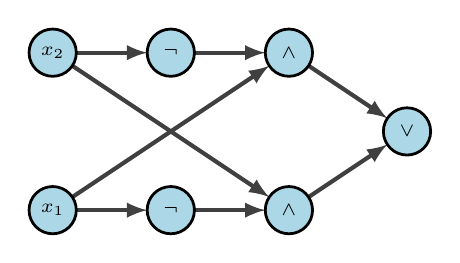
\begin{tikzpicture}
                \Vertex[y=0,x=0,label=$x_1$]{x1}
                \Vertex[y=2,x=0,label=$x_2$]{x2}
                \Vertex[y=0,x=1.5,label=$\neg$]{nx1}
                \Vertex[y=2,x=1.5,label=$\neg$]{nx2}
                \Vertex[y=0,x=3,label=$\land$]{ax1}
                \Vertex[y=2,x=3,label=$\land$]{ax2}
                \Vertex[y=1,x=4.5,label=$\lor$]{end}
                \Edge[Direct](x1)(nx1)
                \Edge[Direct](x2)(nx2)
                \Edge[Direct](nx1)(ax1)
                \Edge[Direct](x2)(ax1)
                \Edge[Direct](nx2)(ax2)
                \Edge[Direct](x1)(ax2)
                \Edge[Direct](ax1)(end)
                \Edge[Direct](ax2)(end)
            \end{tikzpicture}
        \end{figure}

    \defitem{Полный базис. Примеры полных и неполных базисов.}

        \textbf{Полным базисом} называется набор связок, если через эти связки выражается любая булева функция.

        \textbf{Стандартным базисом} назовём набор из операций конъюнкция (И), дизъюнкция (ИЛИ) и отрицание (НЕ).

        Примеры полных базисов:
        \begin{enumerate}
        \item Базис $\{\land, \lor, \neg\}$ полный, так как всякую булеву функцию можно выразить через ДНФ.

        \item Базис $\{\neg, \land\}$ полный, так как $x_1 \lor x_2 = \neg(\neg x_1 \land \neg x_2)$.

        \item Базис $\{\neg, \lor\}$ полный, так как $x_1 \land x_2 = \neg(\neg x_1 \lor \neg x_2)$.

        \item Базис $\{\mid\}$ (штрих Шеффера) полный, так как $\neg x = x \mid x$ и $x_1 \land x_2 = \neg(x_1 \mid x_2) = (x_1 \mid x_2) \mid (x_1 \mid x_2)$.

        \item Базис $\{1, \oplus, \land\}$ полный, так как всякую булеву функцию можно выразить многочленом Жегалкина.
        \end{enumerate}

        Примеры неполных базисов:
        \begin{enumerate}
            \item Базис $\{\land, \lor\}$ неполный, так как он монотонный.

            \item Базис $\{\oplus, \land\}$.

            \item Базис $\{\lor, \to\}$.
        \end{enumerate}

    \defitem{Полином Жегалкина (в стандартном виде).}

        \textbf{Многочленом Жегалкина} называется формула вида
        \begin{equation*}
            \bigoplus_{S \subseteq \{1, \dots, n\}} a_S \bigwedge_{i \in S} x_i, \quad a_S \in \{0, 1\}.
        \end{equation*}

        Примеры многочлена Жегалкина:
        \[\begin{gathered}
            1 \oplus x_1 \oplus x_2 \oplus x_3 \oplus (x_1 \land x_2) \oplus (x_1 \land x_3) \oplus (x_2 \land x_3) \oplus (x_1 \land x_2 \land x_3); \\
            x_3 \oplus (x_1 \land x_3) \oplus (x_2 \land x_3) \oplus (x_1 \land x_2 \land x_3).
        \end{gathered}\]

        Для простоты чтения $\land$ можно опускать:
        \begin{equation*}
            1 \oplus x_1 \oplus x_2 \oplus x_3 \oplus x_1 x_2 \oplus x_1 x_3 \oplus x_2 x_3 \oplus x_1 x_2 x_3; \\
        \end{equation*}

    \defitem{Схемная сложность функции (размер схемы).}

        \textbf{Схемная сложность} булева отображения $f: \{0, 1\}^n \to \{0, 1\}^m$ (в частности, булевой функции) --- это наименьший размер (количество присваиваний) схемы, вычисляющей это выражение.

    \end{colloq}

    \section{Вопросы на знание доказательств}
    \begin{colloq}
    %\setlength\parindent{20pt}

    \proofitem{Сравнение $ax \equiv 1 \pmod{N}$ имеет решение тогда и только тогда, когда $\text{НОД}(a, N) = 1$.}

        \begin{theorem*}
            Сравнение $ax \equiv 1 \pmod N$ имеет решение тогда и только тогда, когда $\gcd(a, N) = 1$.
        \end{theorem*}

        \begin{proof}
            Докажем теорему в обе стороны.
            \begin{itemize}
            \item $\Leftarrow$: 
                Пусть $\gcd(a, N) = 1$. Следовательно, $\exists k_1, k_2 : k_1 a + k_2 N = 1$ (следует из алгоритма Евклида). Вычислим остаток при делении на $N$ обеих частей:
                \[\begin{gathered}
                    \begin{cases}
                        k_1 a + k_2 N &\equiv k_1 a \pmod N \\
                        1 &\equiv 1 \pmod N
                    \end{cases} \\
                    \Downarrow \\
                    k_1 a \equiv 1 \pmod N.
                \end{gathered}\]

                Следовательно, $k_1$ и есть искомый $x$, при котором $ax \equiv 1 \pmod N$.

            \item $\Rightarrow$:
                Пусть $\exists x : ax \equiv 1 \pmod N$. Тогда $\exists t : ax - tN = 1$. Требуется доказать, что в этом случае $\gcd(a, N) = 1$. Докажем от противного.

                Пусть $\gcd(a, N) = d > 1$. Тогда $\exists k_1, k_2 : a = k_1 d$ и $N = k_2 d$. Подставим эти произведения в выражение
                \begin{equation*}
                    k_1 d x - k_2  d t = 1 \implies d (k_1 x - k_2 t) = 1.
                \end{equation*}

                Это возможно только при $d = 1$. Следовательно, $\gcd(a, N) = 1$.
            \end{itemize}
        \end{proof}

    \proofitem{Малая теорема Ферма.}

        \begin{theorem*}
            Если $p$ --- простое число, то
            \begin{equation*}
                a^{p - 1} \equiv 1 \pmod p
            \end{equation*}
            при любом $a$, не делящемся на $p$.
        \end{theorem*}

        \begin{proof}~

            Сначала докажем нужную для доказательства лемму.

            \begin{lemma*}
                Умножение остатков $1, 2, \dots, p - 1$ на $a$ даст те же остатки, но в другом порядке.
            \end{lemma*}

            \begin{proof}
                Докажем от противного. Пусть нашлись каких-то два числа $ax$ и $ay$, дающих одинаковый остаток при делении на $p$ ($x$, $y$ --- остатки). Тогда $a \cdot (x - y)$ делится на $p$, что невозможно (так как $a$ не делится на $p$). Тогда нет совпадающих остатков, так как произведений и остатков $p - 1$.
            \end{proof}

            Рассмотрим произведение $a, 2a, 3a, \dots, (p - 1)a$. Тогда
            \begin{equation*}
                a \cdot 2a \cdot \dots \cdot (p - 1) a \equiv a^{p - 1} \cdot (p - 1)! \pmod p.
            \end{equation*}

            С другой стороны, по лемме это эквивалентно $(p - 1)!$ по модулю $p$ (произведение остатков в другом порядке). Тогда $a^{p - 1} \equiv 1 \pmod p$, что и требовалось доказать.
        \end{proof}

    \proofitem{Теорема Эйлера.}

        \begin{theorem*}
            Пусть $N > 1$ --- произвольное целое число, а $\phi(N)$ равно количеству остатков среди $0, 1, \dots, N - 1$, взаимно простых с $N$. Пусть $a$ --- один из этих остатков. Тогда
            \begin{equation*}
                a^{\phi(N)} \equiv 1 \pmod N.
            \end{equation*}
        \end{theorem*}

        \begin{proof}
            Заметим, что достаточно рассматривать остаток от деления $a$ на $n$.

            Рассмотрим граф, где каждой вершине соответствует какой-то остаток, взаимно простой с $n$, а ребром из $x$ в $y$ будем называть преобразование $x \mapsto y$. Тогда в графе будет $\phi(n)$ вершин. Так как $a$ взаимно просто с $n$, то
            \begin{itemize}
            \item
                Для каждой вершины графа $x$ получаем, что $ax$ взаимно просто с $n$ (так как $x$ взаимно просто с $n$ по построению). Из этого следует, что всегда возможно провести ребро $x \mapsto ax$, если его нет.

            \item
                Уравнение $ax \equiv b \pmod n$ имеет единственное решение (по модулю $n$) для любого $b$. Из этого следует, что из каждой вершины графа выходит ровно одно ребро и в каждую вершину входит ровно одно ребро.
            \end{itemize}

            Тогда граф обязан разбиться на циклы, так как иначе процесс умножения можно продолжать сколь угодно долго и условие на количество ребер нарушится. 
            
            Пусть $k$ --- степень такая, что $a^k \equiv 1 \pmod n$. Заметим, что она существует, так как для единицы существует цикл:
            \begin{equation*}
                1 \mapsto a \mapsto a^2 \mapsto \dots \mapsto a^k.
            \end{equation*}

            Докажем, что все циклы имеют одинаковую длину. Очевидно, что длину, большую $k$ цикл иметь не может (так как $b \cdot a^k \equiv b \pmod n$ и цикл замкнётся). Пусть для какого-то $b$ есть цикл длины $l < k$.

            Тогда $b \cdot a^l \equiv b \pmod n$ и (так как $b$ взаимно просто с $n$, то у него есть обратный элемент) $a^l \equiv 1 \pmod n$.

            Приходим к противоречию. Тогда $\phi(n) = km$ для какого-то $m$ и
            \begin{equation*}
                a^{\phi(n)} \equiv a^{km} \equiv 1^m = 1 \pmod n,
            \end{equation*}
            что и требовалось доказать.
        \end{proof}

    \proofitem{Корректность алгоритма Евклида и расширенного алгоритма Евклида.}
    \proofitem{Основная теорема арифметики.}

        \begin{theorem*}
            Всякое целое положительное число, большее $1$, разлагается на простые множители, причём единственным образом: любые два разложения отличаются только перестановкой сомножителей.
        \end{theorem*}

        \begin{proof}~

            \begin{itemize}
            \item \textbf{Существование}.
                Докажем существование разложения числа $n$ на простые множители, предполагая, что оно уже доказано для любого другого числа, меньшего $n$. Если $n$ --- простое, то существование доказано. Если $n$ --- составное, то оно может быть представлено в виде произведения двух чисел $a$ и $b$, каждое из которых больше $1$, но меньше $n$. Числа $a$ и $b$ либо являются простыми, либо могут быть разложены в произведение простых (уже доказано ранее). Подставив их разложение в $n = a \cdot b$, получим разложение исходного числа $n$ на простые.

            \item \textbf{Единственность}.
                Пусть некоторое число $N$ имеет два разложения:
                \begin{equation*}
                    N = p_1 \cdot p_2 \cdot \dots \cdot p_n = q_1 \cdot q_2 \cdot \dots \cdot q_m.
                \end{equation*}

                Сократим общие сомножители, если они есть. Если сократится не всё, то получим два разложения одного числа, не имеющих общих сомножителей (для удобства оставим $n$ и $m$):
                \begin{equation*}
                    p_1 \cdot p_2 \cdot \dots \cdot p_n = q_1 \cdot q_2 \cdot \dots \cdot q_m.
                \end{equation*}

                Докажем следующее утверждение: если $p$ --- простое число, то произведение чисел, каждое из которых не делится на $p$, не может делиться на $p$. Действительно, если $a \not\equiv 0 \pmod p$ и $b \not\equiv 0 \pmod p$, то и $a \cdot b \not\equiv 0 \pmod p$.

                Правая часть равенства выше --- это произведение чисел, каждое из которых не делится на $p_1$, следовательно, все произведение не делится на $p_1$. Приходим к противоречию, когда $q_1 \cdot \dots \cdot q_m = n$, но $n \not\equiv 0 \pmod{p_1}$. Следовательно, разложение числа $N$ на простые множители единственно.
            \end{itemize}
        \end{proof}

    \proofitem{Китайская теорема об остатках.}

        \begin{theorem*}
            Пусть числа $m_1, m_2, \dots, m_k$ попарно взаимно просты. Рассмотрим следующую систему сравнений:
            \begin{equation*}
                \begin{cases}
                    x \equiv a_1 \pmod{m_1} \\
                    x \equiv a_2 \pmod{m_2} \\
                    \dots \\
                    x \equiv a_k \pmod{m_k} \\
                \end{cases}
            \end{equation*}

            Определим целые числа $M, M_i, b_I$ следующим образом:
            \begin{equation*}
                M = \prod_{i = 1}^k a_i; \quad
                M_i = \dfrac{M}{m_i}; \quad
                M_i \cdot b_i \equiv a_i \pmod{m_i}, 1 \leq i \leq k.
            \end{equation*}

            После чего определим $x_0$ следующим образом:
            \begin{equation*}
                x_o = \sum_{i = 1}^k M_i \cdot b_i.
            \end{equation*}

            Тогда множество целых чисел, удовлетворяющих системе сравнений, составляет класс вычетов $x \equiv x_0 \pmod M$.
        \end{theorem*}

        \begin{proof}
            Так как $\gcd(M_i, m_i) = 1$ по построению, то $b_i$ обязательно существует и $x_0$ также существует.

            Покажем, что $x_0$ соответствует системе сравнений. Так как $m_i \mid M_j$ при $j \neq i$, то $x_0 \equiv M_i \cdot b_i \equiv a_i \pmod{m_i}$ для $1 \leq i \leq k$. Тогда систему можно переписать в следующем виде:
            \begin{equation*}
                 \begin{cases}
                    x \equiv x_0 \pmod{m_1} \\
                    x \equiv x_0 \pmod{m_2} \\
                    \dots \\
                    x \equiv x_0 \pmod{m_k} \\
                \end{cases}
            \end{equation*}

            Тогда $m_i \mid (x - x_0)$ при $1 \leq i \leq k$. Так как все $m_i$ попарно взаимно просты, то эти сравнения будут верны только для тех $x$, что $M \mid (x - x_0)$, что равносильно $x \equiv x_0 \pmod M$.
        \end{proof}

    \proofitem{Мультипликативность функции Эйлера. Формула для функции Эйлера.}
    \proofitem{Формула Байеса. Формула полной вероятности.}
    \proofitem{Парадокс дней рождения (математическое ожидание числа людей с совпавшими днями рождения)}

        Рассмотрим $n$ случайных людей и посмотрим на количество совпадений дней рождения у них, то есть на количество пар людей, имеющих день рождения в один день. Каким в среднем будет это число?

    Сформулируем вопрос точно. Вероятностное пространство: всюду определённая функция из $n$-элементного множества людей $\{x_1, \dots, x_n\}$ в $365$-элементное множество дней в году. Все исходы равновозможные. 
    
    Обозначим случайную величину, равную количеству пар людей с совпадающими днями рождения, через $\xi$. Нам требуется посчитать математическое ожидание случайной величины $\xi$. Но при этом случайная величина довольно сложная, и подсчитывать математическое ожидание непосредственно из определения трудно.
    
    Идея состоит в следующем: давайте разобьём сложную случайную величину $\xi$ в сумму нескольких простых случайных величин. Тогда мы сможем подсчитать отдельно математические ожидания всех простых величин, а затем, пользуясь линейностью математического ожидания, просто сложить результаты.
 
    Обозначим через $I_{ij}$ случайную величину, равную $1$, если у людей $x_i$ и $x_j$ дни рождения совпадают, и равную $0$ в противном случае. Тогда можно заметить, что
    \begin{equation*}
        \xi = \sum_{i < j} I_{ij}.
    \end{equation*}

    Подсчитаем математическое ожидание случайной величины $I_{ij}$. Нетрудно увидеть, что вероятность того, что у двух случайных людей дни рождения совпадают, равна $\dfrac{1}{365}$, так что с вероятностью $\dfrac{1}{365}$ случайная величина равна $1$, и с вероятностью $1 - \dfrac{1}{365}$ равна $0$.

    Получаем, что $\E[I_{ij}] = \dfrac{1}{365}$ (для всякой пары $i$, $j$). Для математического ожидания $\xi$ из линейности получаем
    \begin{equation*}
        \E[\xi] = \E\left[\sum_{i < j} I_{ij}\right] = \sum_{i < j} 1 \cdot \dfrac{1}{365} = \dfrac{n \cdot (n - 1)}{2 \cdot 365}.
    \end{equation*}

    Например, если число людей $n$ больше $27$, то $E[\xi] > 1$, то есть естественно ожидать, что будет не меньше одного совпадения дней рождения.

    \proofitem{Неравенство Маркова.}
    \proofitem{Нижняя оценка на максимальное количество ребер в разрезе.}
    \proofitem{Любое бесконечное множество содержит счётное подмножество. Любое подмножество счётного множества конечно или счётно.}
    \proofitem{Конечное или счётное объединение конечных или счётных множеств конечно или счётно}
    \proofitem{Счётность декартова произведения счетных множеств. Счётность множества рациональных чисел.}
    \proofitem{Равномощность отрезков, интервалов, лучей и прямых (явные биекции).}
    \proofitem{Несчетность множества бесконечных двоичных последовательностей.}
    \proofitem{Теорема Кантора-Бернштейна.}
    \proofitem{Нижняя оценка на число монотонных булевых функций: монотонных булевых функций от $2n$ переменных не меньше $2^{\frac{2^n}{2n + 1}}$}
    \proofitem{Существование и единственность полинома Жегалкина (в стандартном виде) для любой булевой функции.}
    \proofitem{Разложение в ДНФ и КНФ булевой функции.}
    \proofitem{Верхняя оценка $O(n 2^n)$ схемной сложности булевой функции от $n$ переменных.}
    \proofitem{Булевы схемы для сложения и умножения n-битовых чисел. Оценка размера.}
    \proofitem{Булева схема для задачи о связности графа. Оценка размера.}
    \proofitem{Задача об угадывании числа. Верхняя и нижняя оценки.}
    \proofitem{Задача о сортировке нижняя оценка.}
    \proofitem{Задача о нахождении самой тяжелой монеты. Верхние и нижние оценки.}

    \end{colloq}

\end{document}